%%%%%%%%%%%%%%%%%%%%%%%%%%%%%%%%%%%%%%%%%
% Lachaise Assignment
% LaTeX Template
% Version 1.0 (26/6/2018)
%
% This template originates from:
% http://www.LaTeXTemplates.com
%
% Authors:
% Marion Lachaise & François Févotte
% Vel (vel@LaTeXTemplates.com)
%
% License:
% CC BY-NC-SA 3.0 (http://creativecommons.org/licenses/by-nc-sa/3.0/)
% 
%%%%%%%%%%%%%%%%%%%%%%%%%%%%%%%%%%%%%%%%%

%----------------------------------------------------------------------------------------
%	PACKAGES AND OTHER DOCUMENT CONFIGURATIONS
%----------------------------------------------------------------------------------------

\documentclass{article}
\usepackage{float}

%%%%%%%%%%%%%%%%%%%%%%%%%%%%%%%%%%%%%%%%%
% Lachaise Assignment
% Structure Specification File
% Version 1.0 (26/6/2018)
%
% This template originates from:
% http://www.LaTeXTemplates.com
%
% Authors:
% Marion Lachaise & François Févotte
% Vel (vel@LaTeXTemplates.com)
%
% License:
% CC BY-NC-SA 3.0 (http://creativecommons.org/licenses/by-nc-sa/3.0/)
% 
%%%%%%%%%%%%%%%%%%%%%%%%%%%%%%%%%%%%%%%%%

%----------------------------------------------------------------------------------------
%	PACKAGES AND OTHER DOCUMENT CONFIGURATIONS
%----------------------------------------------------------------------------------------

\usepackage{amsmath,amsfonts,stmaryrd,amssymb} % Math packages

\usepackage{enumerate} % Custom item numbers for enumerations

\usepackage[ruled]{algorithm2e} % Algorithms

\usepackage[framemethod=tikz]{mdframed} % Allows defining custom boxed/framed environments

\usepackage{listings} % File listings, with syntax highlighting
\lstset{
	basicstyle=\ttfamily, % Typeset listings in monospace font
}

%----------------------------------------------------------------------------------------
%	DOCUMENT MARGINS
%----------------------------------------------------------------------------------------

\usepackage{geometry} % Required for adjusting page dimensions and margins

\geometry{
	paper=a4paper, % Paper size, change to letterpaper for US letter size
	top=2.5cm, % Top margin
	bottom=3cm, % Bottom margin
	left=2.5cm, % Left margin
	right=2.5cm, % Right margin
	headheight=14pt, % Header height
	footskip=1.5cm, % Space from the bottom margin to the baseline of the footer
	headsep=1.2cm, % Space from the top margin to the baseline of the header
	%showframe, % Uncomment to show how the type block is set on the page
}

%----------------------------------------------------------------------------------------
%	FONTS
%----------------------------------------------------------------------------------------

\usepackage[utf8]{inputenc} % Required for inputting international characters
\usepackage[T1]{fontenc} % Output font encoding for international characters

\usepackage{XCharter} % Use the XCharter fonts

%----------------------------------------------------------------------------------------
%	COMMAND LINE ENVIRONMENT
%----------------------------------------------------------------------------------------

% Usage:
% \begin{commandline}
%	\begin{verbatim}
%		$ ls
%		
%		Applications	Desktop	...
%	\end{verbatim}
% \end{commandline}

\mdfdefinestyle{commandline}{
	leftmargin=10pt,
	rightmargin=10pt,
	innerleftmargin=15pt,
	middlelinecolor=black!50!white,
	middlelinewidth=2pt,
	frametitlerule=false,
	backgroundcolor=black!5!white,
	frametitle={Command Line},
	frametitlefont={\normalfont\sffamily\color{white}\hspace{-1em}},
	frametitlebackgroundcolor=black!50!white,
	nobreak,
}

% Define a custom environment for command-line snapshots
\newenvironment{commandline}{
	\medskip
	\begin{mdframed}[style=commandline]
}{
	\end{mdframed}
	\medskip
}

%----------------------------------------------------------------------------------------
%	FILE CONTENTS ENVIRONMENT
%----------------------------------------------------------------------------------------

% Usage:
% \begin{file}[optional filename, defaults to "File"]
%	File contents, for example, with a listings environment
% \end{file}

\mdfdefinestyle{file}{
	innertopmargin=1.6\baselineskip,
	innerbottommargin=0.8\baselineskip,
	topline=false, bottomline=false,
	leftline=false, rightline=false,
	leftmargin=2cm,
	rightmargin=2cm,
	singleextra={%
		\draw[fill=black!10!white](P)++(0,-1.2em)rectangle(P-|O);
		\node[anchor=north west]
		at(P-|O){\ttfamily\mdfilename};
		%
		\def\l{3em}
		\draw(O-|P)++(-\l,0)--++(\l,\l)--(P)--(P-|O)--(O)--cycle;
		\draw(O-|P)++(-\l,0)--++(0,\l)--++(\l,0);
	},
	nobreak,
}

% Define a custom environment for file contents
\newenvironment{file}[1][File]{ % Set the default filename to "File"
	\medskip
	\newcommand{\mdfilename}{#1}
	\begin{mdframed}[style=file]
}{
	\end{mdframed}
	\medskip
}

%----------------------------------------------------------------------------------------
%	NUMBERED QUESTIONS ENVIRONMENT
%----------------------------------------------------------------------------------------

% Usage:
% \begin{question}[optional title]
%	Question contents
% \end{question}

\mdfdefinestyle{question}{
	innertopmargin=1.2\baselineskip,
	innerbottommargin=0.8\baselineskip,
	roundcorner=5pt,
	nobreak,
	singleextra={%
		\draw(P-|O)node[xshift=1em,anchor=west,fill=white,draw,rounded corners=5pt]{%
		Question \theQuestion\questionTitle};
	},
}

\newcounter{Question} % Stores the current question number that gets iterated with each new question

% Define a custom environment for numbered questions
\newenvironment{question}[1][\unskip]{
	\bigskip
	\stepcounter{Question}
	\newcommand{\questionTitle}{~#1}
	\begin{mdframed}[style=question]
}{
	\end{mdframed}
	\medskip
}

%----------------------------------------------------------------------------------------
%	WARNING TEXT ENVIRONMENT
%----------------------------------------------------------------------------------------

% Usage:
% \begin{warn}[optional title, defaults to "Warning:"]
%	Contents
% \end{warn}

\mdfdefinestyle{warning}{
	topline=false, bottomline=false,
	leftline=false, rightline=false,
	nobreak,
	singleextra={%
		\draw(P-|O)++(-0.5em,0)node(tmp1){};
		\draw(P-|O)++(0.5em,0)node(tmp2){};
		\fill[black,rotate around={45:(P-|O)}](tmp1)rectangle(tmp2);
		\node at(P-|O){\color{white}\scriptsize\bf !};
		\draw[very thick](P-|O)++(0,-1em)--(O);%--(O-|P);
	}
}

% Define a custom environment for warning text
\newenvironment{warn}[1][Warning:]{ % Set the default warning to "Warning:"
	\medskip
	\begin{mdframed}[style=warning]
		\noindent{\textbf{#1}}
}{
	\end{mdframed}
}

%----------------------------------------------------------------------------------------
%	INFORMATION ENVIRONMENT
%----------------------------------------------------------------------------------------

% Usage:
% \begin{info}[optional title, defaults to "Info:"]
% 	contents
% 	\end{info}

\mdfdefinestyle{info}{%
	topline=false, bottomline=false,
	leftline=false, rightline=false,
	nobreak,
	singleextra={%
		\fill[black](P-|O)circle[radius=0.4em];
		\node at(P-|O){\color{white}\scriptsize\bf i};
		\draw[very thick](P-|O)++(0,-0.8em)--(O);%--(O-|P);
	}
}

% Define a custom environment for information
\newenvironment{info}[1][Info:]{ % Set the default title to "Info:"
	\medskip
	\begin{mdframed}[style=info]
		\noindent{\textbf{#1}}
}{
	\end{mdframed}
}
 % Include the file specifying the document structure and custom commands

%----------------------------------------------------------------------------------------
%	ASSIGNMENT INFORMATION
%----------------------------------------------------------------------------------------

\title{Implementation and Changes Notes Based on Software Requirements Specification of Student Attendance Control v0.5  } % Title of the assignment

\author{Arif A. Balik\\ Omer Faruk Can\\ Huseyin Bayraktar } % Author name and email address

\date{Istanbul Arel University --- \today} % University, school and/or department name(s) and a date

%----------------------------------------------------------------------------------------

\begin{document}

\maketitle % Print the title

%----------------------------------------------------------------------------------------
%	INTRODUCTION
%----------------------------------------------------------------------------------------

\section*{Introduction} % Unnumbered section

This document covers changes and implementation notes about Student Attendance Control (SAC). Throughout the document, sections, changes will be compared to Software Requirement Specification (SRS) version 0.5 of SAC. Every change includes some reasoning and technical details along with figures, tables etc.

First, document begins with implementation, this section includes technical detail of system that has been implemented. Then there comes changes section, which refers to the changes that has been made based on SRS v0.5 of the project.

\begin{info} % Information block
	Throughout the document the name `Device' refers to the hardware that reads the student cards and `Web server' refers to web application.
\end{info}

%----------------------------------------------------------------------------------------
%	PROBLEM 1
%----------------------------------------------------------------------------------------

\section{Implementation} % Numbered section

\subsection{The Device}

The device contains a WiFi SoC (System on Chip) ESP8266 with NodeMCU Development Kit, this SoC is the main controller of the device. Also there is a RFID front-end chip connected via SPI (Serial Peripheral Interface), this chip automatically detects a near RFID chip and reads its memory and sends it through SPI to ESP8266;
\begin{file}[Waiting for RFID Card]
\begin{lstlisting}[language=C]
  // Look for new cards
  if ( ! rfid.PICC_IsNewCardPresent())
    return;

  // Verify if the NUID has been readed
  if ( ! rfid.PICC_ReadCardSerial())
    return;
\end{lstlisting}
\end{file}

\begin{figure}
 \begin{center}
	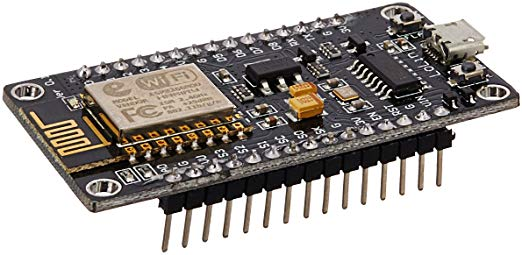
\includegraphics[scale=0.5]{nodemcu}
  	\caption{NodeMCU Dev. Kit}
  \end{center}
\end{figure}

Then, data will be processed and send to the web server. After getting the response ESP8266 will activate a buzzer and leds to show the results.

%------------------------------------------------

\subsection{Web Server}

Web server is mostly is as described in SRS with only small differences. Only missing part is covered in the \textit{Changes} section.

Web server is written in ASP.NET and Visual Studio 2017 as the IDE. 

\begin{figure}[H]
 \begin{center}
	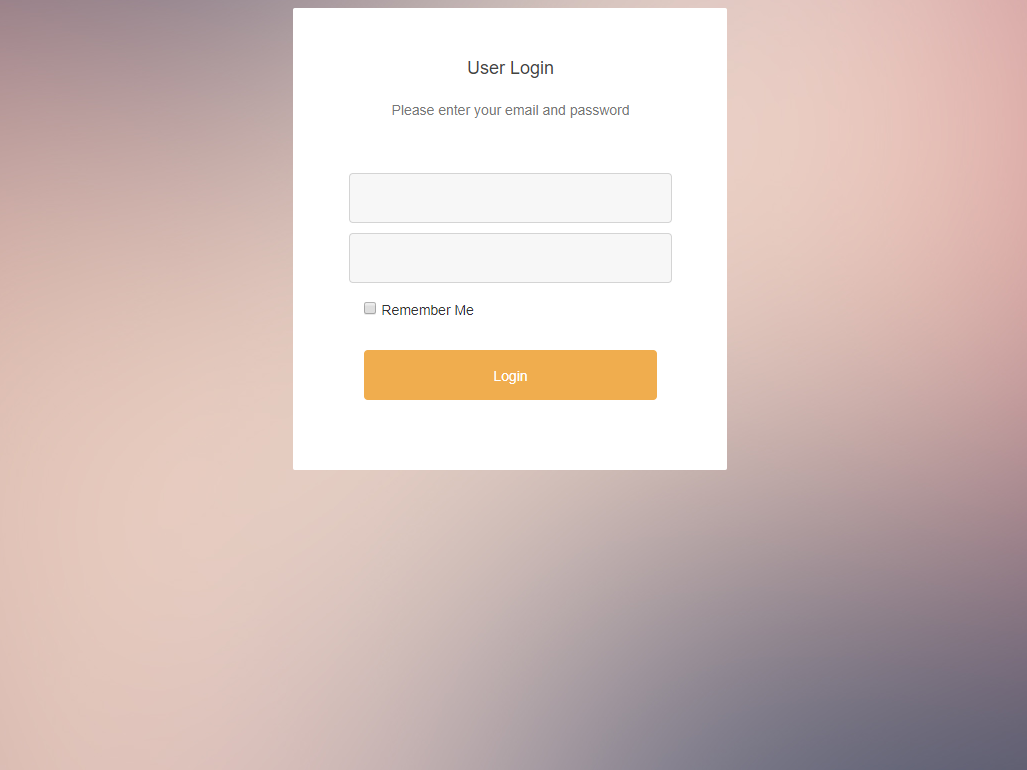
\includegraphics[scale=0.5]{login}
  	\caption{Login page of web server}
  \end{center}
\end{figure}

	
%------------------------------------------------

\section{Changes}

Changes has been made mostly on the device. All of them are listed below;

{\setlength{\parindent}{0cm}
\vspace{5mm}
\textbf{FR-3: Device shall work with WiFi and stand alone when there is no WiFi present}
\vspace{5mm}
}

This has been changed, device is only operational when WiFi is present. Because attendance record should be real-time, and since the processing side is on the web server, there is no need to keep data on the device for later use.

{\setlength{\parindent}{0cm}
\vspace{5mm}
\textbf{FR-5: Device shall read and generate JSON forma \\ SI-3.2: Device shall send every RFID card it detects along with other informations as the following JSON format}
\vspace{5mm}
}

It has been found that using JSON only make things more complicated. Only data device sends to the web server is student card id and class id, thus using JSON for such small array is inefficient. Therefore device is now just uses basic http request, such as;

\begin{file}[HTTP Request]
\begin{lstlisting}[language=C]
[domain].com/out?studentid=[sid]&classid=[cid]
\end{lstlisting}
\end{file}

{\setlength{\parindent}{0cm}
\vspace{5mm}
\textbf{FR-6: Device shall maintain time information within the system with an internal backup battery \\ OE-1: System is dependent on geographical areas. Timezone shall be set before operation}
\vspace{5mm}
}

All the date information is handled in web server.

{\setlength{\parindent}{0cm}
\vspace{5mm}
\textbf{FR-10: Web server shall generate detailed report for every student \\ FE-4:Monitor students individually}
\vspace{5mm}
}

Due to time constraints, it has been removed from functional requirement and features.

{\setlength{\parindent}{0cm}
\vspace{5mm}
\textbf{FR-7: When on battery device shall monitor its battery status and inform its environment when battery is running out.}
\vspace{5mm}
}

Due to time constraints ,it has been we removed from functional requirement.

{\setlength{\parindent}{0cm}
\vspace{5mm}
\textbf{NFP-4: Device shall establish a communication channel with \%95 percent success rate.}
\vspace{5mm}
}

It has been removed, since there is not enough time to test such a thing.

{\setlength{\parindent}{0cm}
\vspace{5mm}
\textbf{FE-1:Data and application hosting on Amazon web servers}
\vspace{5mm}
}

This feature is removed because of budget constraints.

{\setlength{\parindent}{0cm}
\vspace{5mm}
\textbf{MCU: ST STM32F0}
\vspace{5mm}
}

This specification is removed because WiFi SoC can handle the job of MCU.

{\setlength{\parindent}{0cm}
\vspace{5mm}
\textbf{RTC: Dallas Semi. DS1307}
\vspace{5mm}
}

This specification is removed because device won't keep date information.

\newpage
\section*{Licence}
\begin{verbatim}

    Student Attendance Control. This project aims to keep student attendance data autonomously.
    Copyright (C) 2019  Arif A. Balik, Huseyin Bayraktar, Omer F. Can

    This program is free software: you can redistribute it and/or modify
    it under the terms of the GNU General Public License as published by
    the Free Software Foundation, either version 3 of the License, or
    (at your option) any later version.

    This program is distributed in the hope that it will be useful,
    but WITHOUT ANY WARRANTY; without even the implied warranty of
    MERCHANTABILITY or FITNESS FOR A PARTICULAR PURPOSE.  See the
    GNU General Public License for more details.

    You should have received a copy of the GNU General Public License
    along with this program.  If not, see <https://www.gnu.org/licenses/>

\end{verbatim}
%----------------------------------------------------------------------------------------

\end{document}
